\section{Datensatz}
\label{chap:3-Datensatz}
Analog zu der in Kapitel \ref{chap:vorherige-arbeiten-rub} beschriebenen Arbeit verwendet diese Studienarbeit den \ac{GTSRB} als Datensatz. Dass dies der größte veröffentlichte Datensatz für deutsche Straßenschilder ist, stellt hierbei den ausschlaggebenden Punkt dar.

Die Bilder des \ac{GTSRB} verteilen sich auf 43 Klassen respektive 43 verschiedene Arten von Straßenschildern. Eine Auflistung aller Klassen ist im Anhang in Abbildung \ref{fig:all-pictograms} dargestellt. Beispielbilder aus dem \ac{GTSRB} zeigt Abbildung \ref{fig:gtrsb-paper-bsp-images}: \cite{GTSRB}


\begin{figure}[H]
   \centering
   \begin{subfigure}[b]{0.125\textwidth}
       \centering
       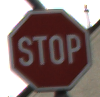
\includegraphics[height=\textwidth]{../images/GTSRB/00093.png}
       \caption{}
       \label{fig:gtrsb-paper-bsp-image-1}
   \end{subfigure}
   \hspace{3em}%
   \begin{subfigure}[b]{0.125\textwidth}
       \centering
       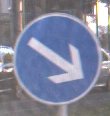
\includegraphics[height=\textwidth]{../images/GTSRB/00847.png}
       \caption{}
       \label{fig:gtrsb-paper-bsp-image-2}
   \end{subfigure}
   \hspace{3em}%
   \begin{subfigure}[b]{0.125\textwidth}
       \centering
       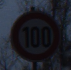
\includegraphics[height=\textwidth]{../images/GTSRB/00040.png}
       \caption{}
       \label{fig:gtrsb-paper-bsp-image-3}
   \end{subfigure}
   \hspace{3em}%
   \begin{subfigure}[b]{0.125\textwidth}
    \centering
    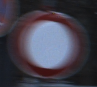
\includegraphics[height=\textwidth]{../images/GTSRB/00052.png}
    \caption{}
    \label{fig:gtrsb-paper-bsp-image-4}
\end{subfigure}
      \caption{Beispielbilder aus dem \acs{GTSRB} Datensatz \cite{GTSRB}}
      \label{fig:gtrsb-paper-bsp-images}
\end{figure}

Der \ac{GTSRB} setzt sich aus Bildern zusammen, die unterschiedliche Seitenverhältnisse und verschiedene Auflösungen besitzen. Ein Großteil davon ist kleiner als 100x100 Pixel. Auf jedem Bild ist genau ein Straßenschild zu sehen. Die Bilder basieren auf Videos, die durch die Autoren tagsüber im Straßenverkehr aufgenommen wurden. Dabei sind die Trainingsbilder ungleich auf die Anzahl an Klassen verteilt. Dies hängt mitunter damit zusammen, dass die jeweiligen Schilder nicht gleich häufig im Straßenverkehr vorkommen. Zusätzlich zu den Trainingsbildern besitzt der \ac{GTSRB} 12.630 Testbilder, welche in dieser Arbeit zur Evaluation des Modells verwendet werden können. Eine nennenswerte Eigenschaft des \ac{GTSRB} ist, dass eine signifikante Anzahl an Bildern einer Klasse sich ähnlich sehen. Das hängt damit zusammen, dass sie mit zeitlicher Verzögerung aus der selben Fahrsituation stammen. \cite{GTSRB}

Die Bilder, die durch diese Studienarbet generiert werden sollen, haben eine Auflösung von 256x256 Pixel. Auf den genauen Hintergrund hierzu wird zu einem späteren Zeitpunt eingegangen. Unter anderem deshalb ist der \ac{GTSRB} für diese Arbeit zunächst so präpariert, dass nur Bilder verwendet werden, die mindestens 50 Pixel breit oder hoch sind. Dies wird im Verlauf geändert, sodass die Mindestgröße 75 Pixel beträgt. Das verringert die Anzahl an verfügbaren Trainingsbildern signifikant verringert. Der präparierte Datensatz besteht aus 4.510 Bildern, wodurch nur etwa 11\% des \ac{GTSRB} genutzt werden.

Die Verteilung der Daten ist auch im präparierten Datensatz nicht homogen. Das nachfolgende Diagramm zeigt hierfür die Anzahl an Trainingsbildern pro Klasse.

\definecolor{plotcolor}{HTML}{2b2b2b}
\definecolor{chinesedata}{HTML}{009F93}
\definecolor{mapillary}{HTML}{FF6542}

\begin{figure}[H]
\centering
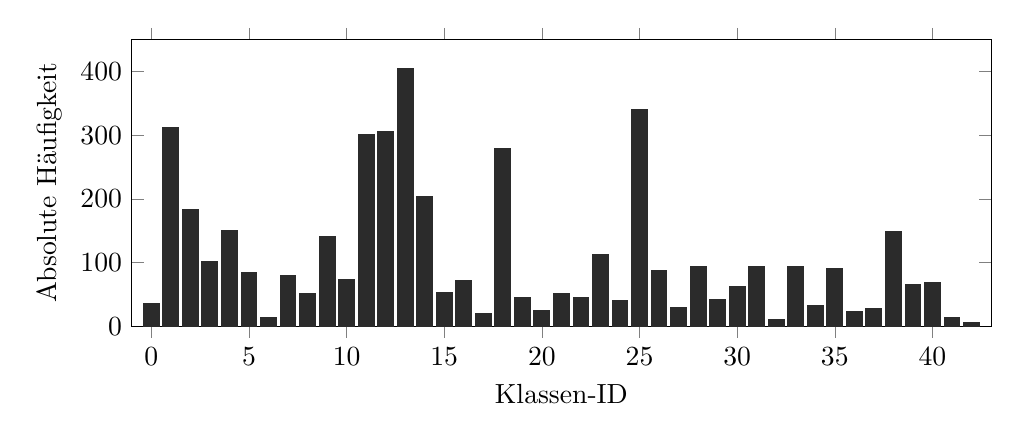
\begin{tikzpicture}
    \begin{axis} [ybar, ylabel={Absolute Häufigkeit}, xlabel={Klassen-ID}, width=\linewidth*0.9, height=\linewidth*0.3, scale only axis=true, xmin=-1, xmax=43, ymin=0, ymax=450, bar width=0.2cm, ytick={0, 100, 200, 300, 400}]
    \addplot[plotcolor, fill] coordinates {
        (0, 36) %(0, 40)
        (1, 312) %(1, 390) 
        (2, 184) %(2, 270)
        (3, 102) 
        (4, 150) %(3, 127)
        (5, 84) %(4, 192)
        (6, 13) %(5, 113)
        (7, 80) %(7, 101)
        (8, 52) %(8, 69)
        (9, 141) %(11, 396)
        (10, 73) %(18, 342)
        (11, 301) %(19, 56)
        (12, 306) %(20, 31)
        (13, 405) %(21, 70)
        (14, 203) %(22, 58)
        (15, 53) %(23, 144)
        (16, 71) %(24, 75)
        (17, 20) %(25, 451)
        (18, 279) %(26, 118)
        (19, 45) %(27, 62)
        (20, 24) %(28, 126)
        (21, 51) %(29, 60)
        (22, 45) %(30, 71)
        (23, 112) %(31, 117)
        (24, 40) %(6, 14)
        (25, 341) %(9, 214)
        (26, 88) %(10, 110)
        (27, 29) %(12, 424)
        (28, 93) %(13, 534)
        (29, 42) %(14, 269)
        (30, 63) %(15, 77)
        (31, 93) %(16, 85)
        (32, 10) %(17, 21)
        (33, 94) %(32, 12)
        (34, 33) %(33, 116)
        (35, 90) %(34, 39)
        (36, 23) %(35, 121)
        (37, 28) %(36, 53)
        (38, 148) %(37, 31)
        (39, 66) %(38, 195)
        (40, 68) %(39, 87)
        (41, 14) %(40, 88)
        (42, 5) %(41, 19)
                 %(42, 10)
    };
    \end{axis}
\end{tikzpicture}
\caption{Häufigkeitsverteilung der Klassen von Straßenschildern im präparierten \ac{GTSRB}}
\end{figure}

Eine ungleiche Verteilung der Trainingsdaten kann die Qualität der generierten Bilder negativ beeinflussen. Die in Kapitel \ref{chap:vorherige-arbeiten-rub} beschriebene Veröffentlichung gibt hierauf bereits Hinweise \cite{gtsrbGAN}. Aus diesem Grund, und da die Größe des präparierten Datensatzes als zu gering bewertet werden kann, ist der Datensatz derart erweitert, dass er einerseits mehr Trainingsbilder enthält und andererseits eine gleichmäßigere Verteilung der Klassen vorliegt. Dabei wird nicht darauf geachtet, jede einzelne Klasse möglichst gleich oft zu repräsentieren, sondern jede Kategorie von Klassen. Die 43 Klassen werden dazu in die Kategorien \emph{Geschwindigkeitsbegrenzungen}, \emph{Richtungsweiser}, \emph{Aufhebungen}, \emph{Verbotszeichen}, \emph{Gefahrzeichen} und \emph{Einzigartig} unterteilt. Es zeigt sich nämlich, dass das Modell zwischen Straßenschildern, die eine ähnliche Bedeutung und damit auch äußerliche Ähnlichkleiten besitzen, recht gut transferieren kann. Diese Einteilung der Schilder in unterschiedliche Kategorien erfolgt auch in der ursprünglichen Veröffentlichung des \ac{GTSRB}. Die Kategorisierung für diese Studienarbeit ist identisch, verwendet jedoch deutschen Bezeichnungen für die Kategorien. Im Anhang befindet sich eine übersicht über die Kategorien von Schildern und ihre zugeordneten Klassen.

Der Großteil an hinzugefügten Trainingsdaten stammt aus der chinesischen \emph{Traffic Sign Recognition Database}, die ein Teil der \emph{Chinese Traffic Sign Database} ist. Dieser Datensatz ist bedeutend kleiner als der \ac{GTSRB}, bietet jedoch auch einige Bilder mit einer höheren Auflösung als der \ac{GTSRB}. Somit ist  hier ein größerer Anteil des Datensatzes nutzbar. Allgemein ähneln diese Bildern denen des \ac{GTSRB}. Mit dem Unterschied, dass sie chinesische Straßenschilder zeigen. Für den präparierten Datensatz werden nur die Bilder verwendet, die in eine der genannten Kategorien fallen. Nachfolgend sind Beispielsbilder aus dem Datensatz dargestellt: \cite{chinese-dataset}


\begin{figure}[H]
    \centering
    \begin{subfigure}[b]{0.125\textwidth}
        \centering
        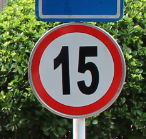
\includegraphics[height=\textwidth]{../images/3 Konzeption des Generative Adversarial Networks/Chinese Dataset/001_0013.png}
        \caption{}
    \end{subfigure}
    \hspace{3em}%
    \begin{subfigure}[b]{0.125\textwidth}
        \centering
        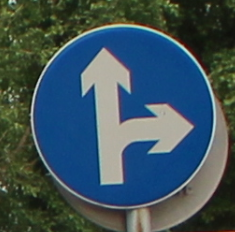
\includegraphics[height=\textwidth]{../images/3 Konzeption des Generative Adversarial Networks/Chinese Dataset/020_0005.png}
        \caption{}
    \end{subfigure}
    \hspace{3em}%
    \begin{subfigure}[b]{0.125\textwidth}
        \centering
        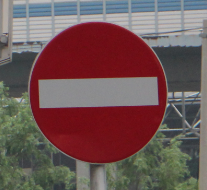
\includegraphics[height=\textwidth]{../images/3 Konzeption des Generative Adversarial Networks/Chinese Dataset/055_1_0029.png}
        \caption{}
    \end{subfigure}
    \hspace{3em}%
    \begin{subfigure}[b]{0.125\textwidth}
     \centering
     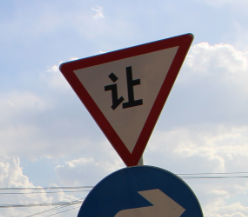
\includegraphics[height=\textwidth]{../images/3 Konzeption des Generative Adversarial Networks/Chinese Dataset/056_1_0015.png}
     \caption{}
 \end{subfigure}
       \caption{Beispielbilder aus der chinesischen Traffic Sign Recognition Database \cite{chinese-dataset}}
       \label{fig:chinese-dataset-bsp-images}
 \end{figure}

Zu sehen ist in Abbildung \ref{fig:chinese-dataset-bsp-images} eine Geschwindigkeitsbegrenzung, ein Richtungsweiser, ein Verbotszeichen und ein Schild der Kategorie \emph{Einzigartig}. Der präparierte Datensatz beinhaltet auch Schilder, die nicht durch das Modell dieser Studienarbeit generiert werden sollen. Wie etwa die in Abbildung \ref{fig:chinese-dataset-bsp-images} vorhandene Geschwindigkeitsbegrenzung von 15$\frac{km}{h}$. Die Idee ist, dass das Modell diese Bilder dennoch nutzen kann, um die Generierung von anderen Geschwindigkeitsbegrenzungen zu optimieren. Es sind allgemein Unterschiede zu deutschen Straßenschildern vorhanden, die jedoch in dieser Arbeit als vernachlässigbar angenommen werden. Zumindest dann, wenn deutsche Straßenschilder weiterhin den größten Teil des präparierten Datensatzes ausmachen. Eine gewisse Ähnlichkeit ist vorhanden, auch da das Aussehen von Straßenschildern durch das Wiener Übereinkommen über Straßenverkehrszeichen in vielen Ländern weltweit vereinheitlicht ist \cite{vienna-convention}. \cite{chinese-dataset}

Zusätzlich setzt sich der präparierte Datensatz aus Bildern weiterer Datensätze zusammen. Hier ist jedoch die Anzahl an Bildern signifikant geringer als die der chinesischen Traffic Sign Recognition Database. Zwei der Datensätze bestehen aus Bildern, die eine vollständige Sicht außerhalb des Fahrzeugs zeigen. Hier sind demnach gegebenenfalls mehrere Straßenschilder pro Bild zu sehen, wobei zusätzlich andere Fahrzeuge, Gebäude, Personen und weitere Objekte sichtbar sind. Die Datensätze nennen sich \emph{Mapillary Traffic Sign Dataset} und \emph{BelgianTS Dataset} \cite{dataset-mapillary} \cite{dataset-belgiants}.

\begin{figure}[H]
    \centering
    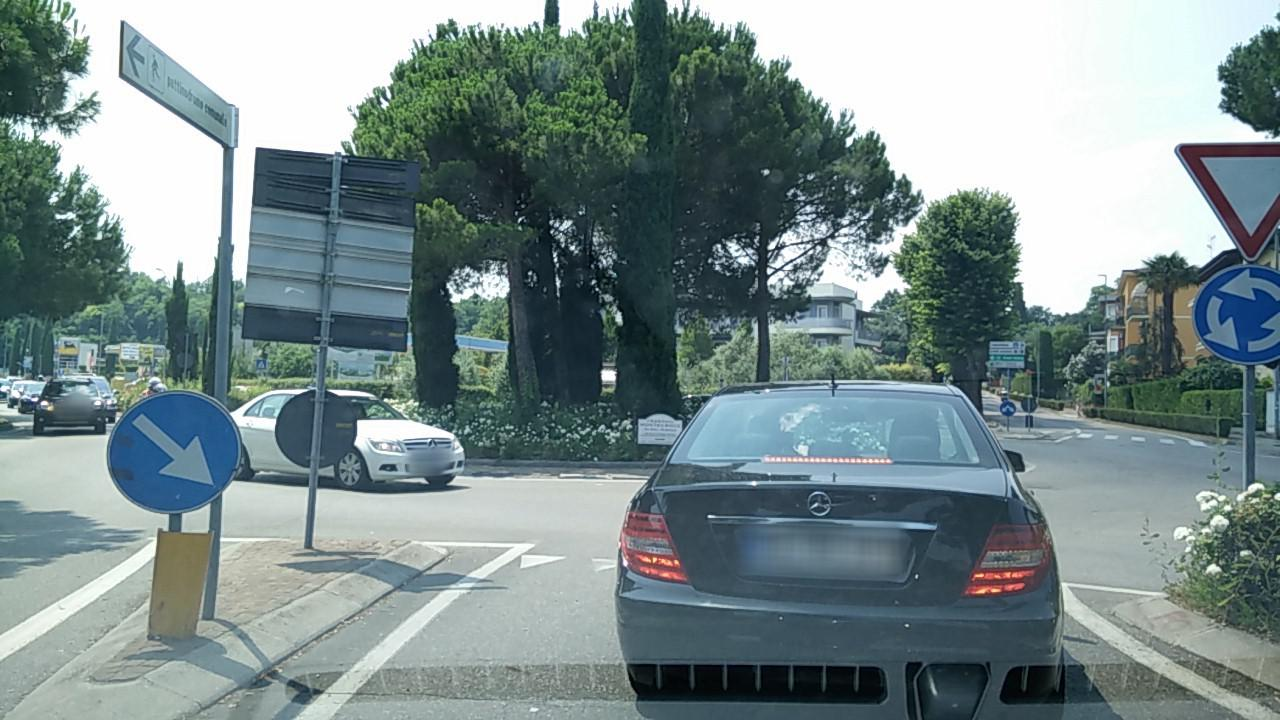
\includegraphics[height=0.3\textwidth]{../images/3 Konzeption des Generative Adversarial Networks/mapillary.jpg}
    \caption{Beispielbild aus dem \emph{Mapillary} Datensatz \cite{dataset-mapillary}}
    \label{fig:full-mapillary-image}
\end{figure}

Da diese Bilder manuell so zugeschnitten werden müssen, dass sie ähnlich zu dem \ac{GTSRB} und der chinesischen Traffic Sign Recognition Database einzelne Schilder mit wenig Hintergrund zeigen, macht diese Menge an Bildern einen geringeren Anteil aus. Aus einem dritten Datensatz werden weniger als 50 Bilder verwendet \cite{dataset-make-ml}. Hier sind größtenteils Stopschildern zu sehen mit einer Bildauflösung von etwa 190 bis zu 300 Pixel in der Höhe oder Breite.

Der vollständige, präparierte Datensatz ist öffentlich unter \href{https://drive.google.com/drive/u/1/folders/1UlZNFEDLymyMFw2BJZcfB2toAIlTVwGb}{\textbf{diesem Link}} verfügbar (Stand: 09.06.2023). Er besteht aus 5.809 Bildern. In der nachfolgenden Abbildung ist die Häufigkeitsverteilung der Trainingsdaten (x-Achse) je Straßenschild-Kategorie (y-Achse) zu sehen. Die drei letztgenannten Datensätze sind in der Farbkodierung der Kategorie \emph{Sonstige} zugeordnet.

\begin{figure}[H]
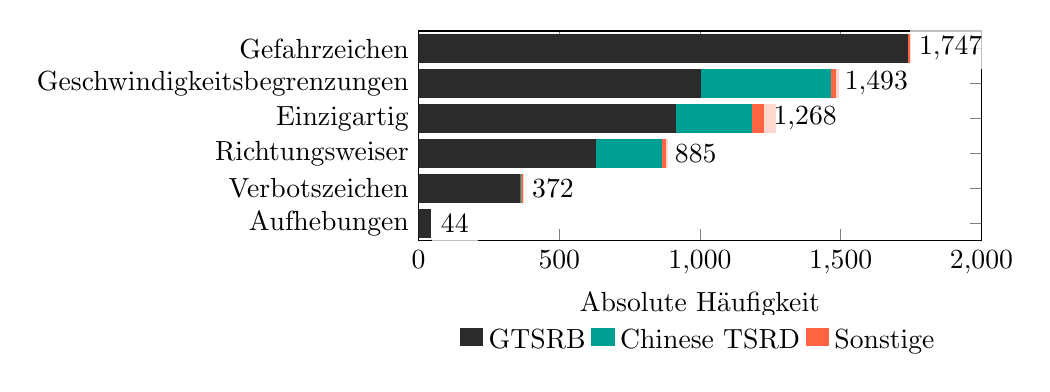
\begin{tikzpicture}
\begin{axis}[ 
xbar stacked, xmin=0, height=\linewidth*0.35, width=\linewidth*0.72,
xlabel={Absolute Häufigkeit},
legend style={at={(0.5,-0.350)}, anchor=north,legend columns=-1, draw=none},
symbolic y coords={
    Aufhebungen, 
    Verbotszeichen,
    Richtungsweiser,
    Einzigartig,
    Geschwindigkeitsbegrenzungen,
    Gefahrzeichen,
    },
ytick=data,
%nodes near coords, 
%nodes near coords align={horizontal},
ytick=data, xmax=2000, xtick={0, 500, 1000, 1500, 2000}
]
\addplot+[plotcolor, fill] coordinates {
    (914,Einzigartig)
    (1000,Geschwindigkeitsbegrenzungen) 
    (630,Richtungsweiser)
    (42,Aufhebungen)
    (358,Verbotszeichen) 
    (1737,Gefahrzeichen)
};
\addplot+[chinesedata, fill] coordinates {
    (268,Einzigartig)
    (463,Geschwindigkeitsbegrenzungen) 
    (234,Richtungsweiser)
    (0,Aufhebungen)
    (4,Verbotszeichen) 
    (0,Gefahrzeichen)
};
\addplot+[mapillary, fill, point meta=x, nodes near coords, nodes near coords align={anchor=west}, every node near coord/.append style={
                black,
                fill=white,
                fill opacity=0.75,
                text opacity=1,
                outer sep=\pgflinewidth % so the label fill doesn't overlap the plot
            }] coordinates {
    (86,Einzigartig)
    (30,Geschwindigkeitsbegrenzungen) 
    (21,Richtungsweiser)
    (2,Aufhebungen)
    (10,Verbotszeichen) 
    (10,Gefahrzeichen)
};
\legend{\strut GTSRB, \strut Chinese TSRD, \strut Sonstige}
\end{axis}
\end{tikzpicture} %width=6cm,height=7.59cm
\caption{Häufigkeitsverteilung der Kategorien von Straßenschildern im präparierten Datensatz}
\end{figure}

Die Kategorie \emph{Aufhebungen} ist nach wie vor signifikant unterrepräsentiert. Eine mögliche Lösung, für die der zeitliche Rahmen nicht ausreicht, wäre, manuell auf \href{https://www.mapillary.com/}{Mapillary} nach solchen Bildern zu suchen. Mapillary ist eine Webseite, auf der Nutzer Bilder zu bestimmten GPS-Koordinaten hochladen können. Das Ziel von Mapillary ist, Straßenansichten für alle Straßen auf der Welt bereitzustellen. Hier ist es möglich, explizit nach bestimmten Arten von Straßenschildern zu suchen. Einer der genannten Datensätze stammt aus einer Mischung von weltweiten Mapillary-Bildern. \cite{dataset-mapillary}
